\subsection*{Interpretability}
%--------------------------------------------------------------------------------------------------
\begin{frame}[t]
    \frametitle{Interpretability}
    \framesubtitle{A paradigmn on interpretable studies}
    \small
    Interpretability approaches have been categorized by two studies 
    \cite{mythos_interp, zhang2021survey}:
    \vspace{-5pt}
    \begin{columns}
        \scriptsize
        \column[T]{.4\textwidth}
        \begin{enumerate}
            \item \textbf{Passive or Active?}\\
            \emph{To add or not modifications to the model.}
        \end{enumerate}
        \column[T]{.6\textwidth}
            \begin{center}
                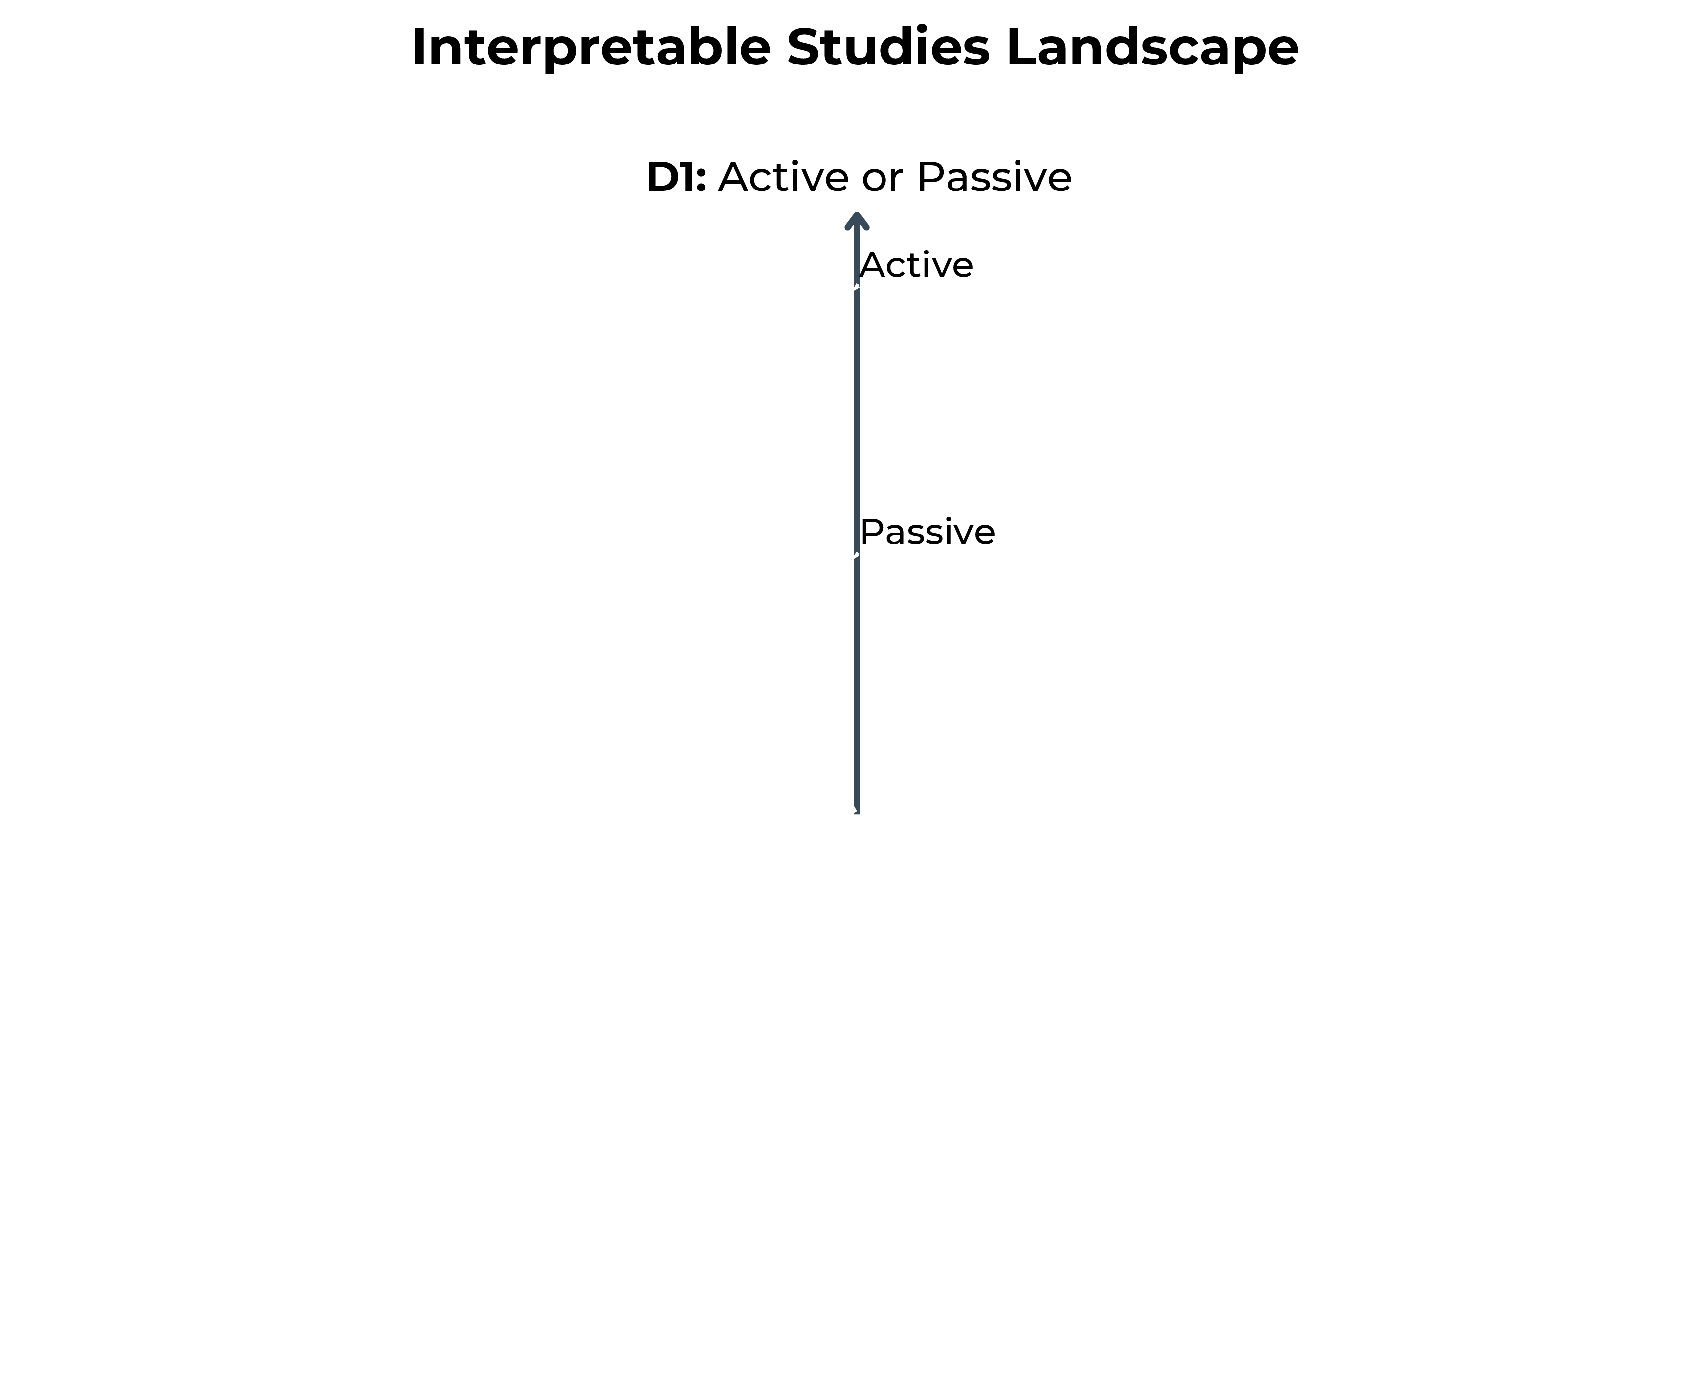
\includegraphics[width=\textwidth]{fig/rel/interp/img/dims/eindim.pdf}
            \end{center}
    \end{columns}
\end{frame}
%--------------------------------------------------------------------------------------------------
\begin{frame}[t]
    \frametitle{Interpretability}
    \framesubtitle{A paradigmn on iterpretable studies}
    \small
    Interpretability approaches have been categorized by two studies 
    \cite{mythos_interp, zhang2021survey}:
    \vspace{-5pt}
    \begin{columns}
        \scriptsize
        \column[T]{.4\textwidth}
        \begin{enumerate}
            \item \textbf{Passive or Active?}\\
            \emph{To add or not modifications to the model.}
            \item \textbf{Type of Explanation}\\
            \emph{Is it an example? An Attribution? Hidden Semantics? Or a Rule?}
        \end{enumerate}
        \column[T]{.6\textwidth}
            \begin{center}
                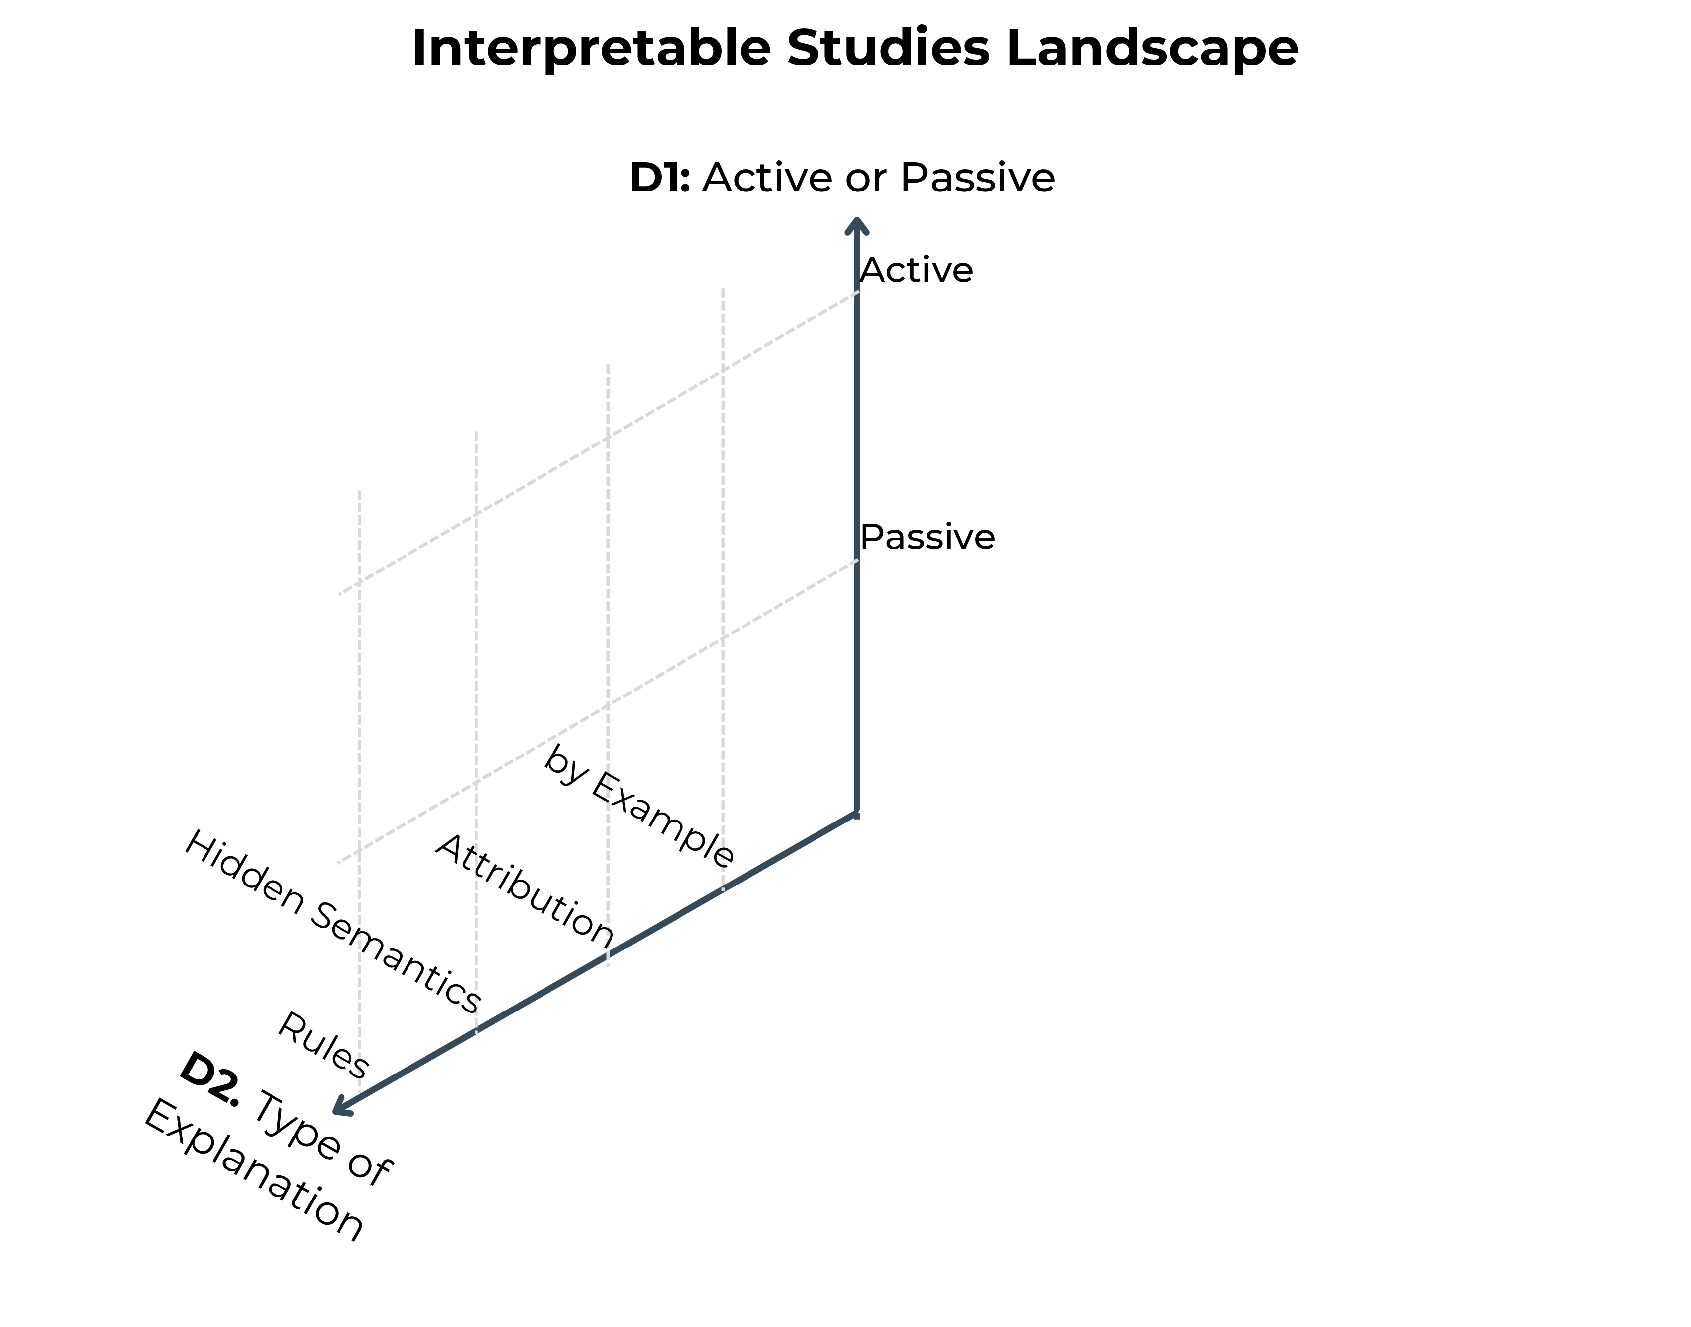
\includegraphics[width=\textwidth]{fig/rel/interp/img/dims/zweidim.pdf}
            \end{center}
    \end{columns}
\end{frame}
%--------------------------------------------------------------------------------------------------
\begin{frame}[t]
    \frametitle{Interpretability}
    \framesubtitle{A paradigmn on iterpretable studies}
    \small
    Interpretability approaches have been categorized by two studies 
    \cite{mythos_interp, zhang2021survey}:
    \vspace{-5pt}
    \begin{columns}
        \scriptsize
        \column[T]{.4\textwidth}
        \begin{enumerate}
            \item \textbf{Passive or Active?}\footnotemark\\
            \emph{To add or not modifications to the model.}
            \item \textbf{Type of Explanation}\\
            \emph{Is it an example? An Attribution? Hidden Semantics? Or a Rule?}
            \item \textbf{Local or Global?}\\
            \emph{Is it a brief explanation? Does it cover more data/ of the model? Does it explain
            the model/data entirely?}
        \end{enumerate}
        \column[T]{.6\textwidth}
            \begin{center}
                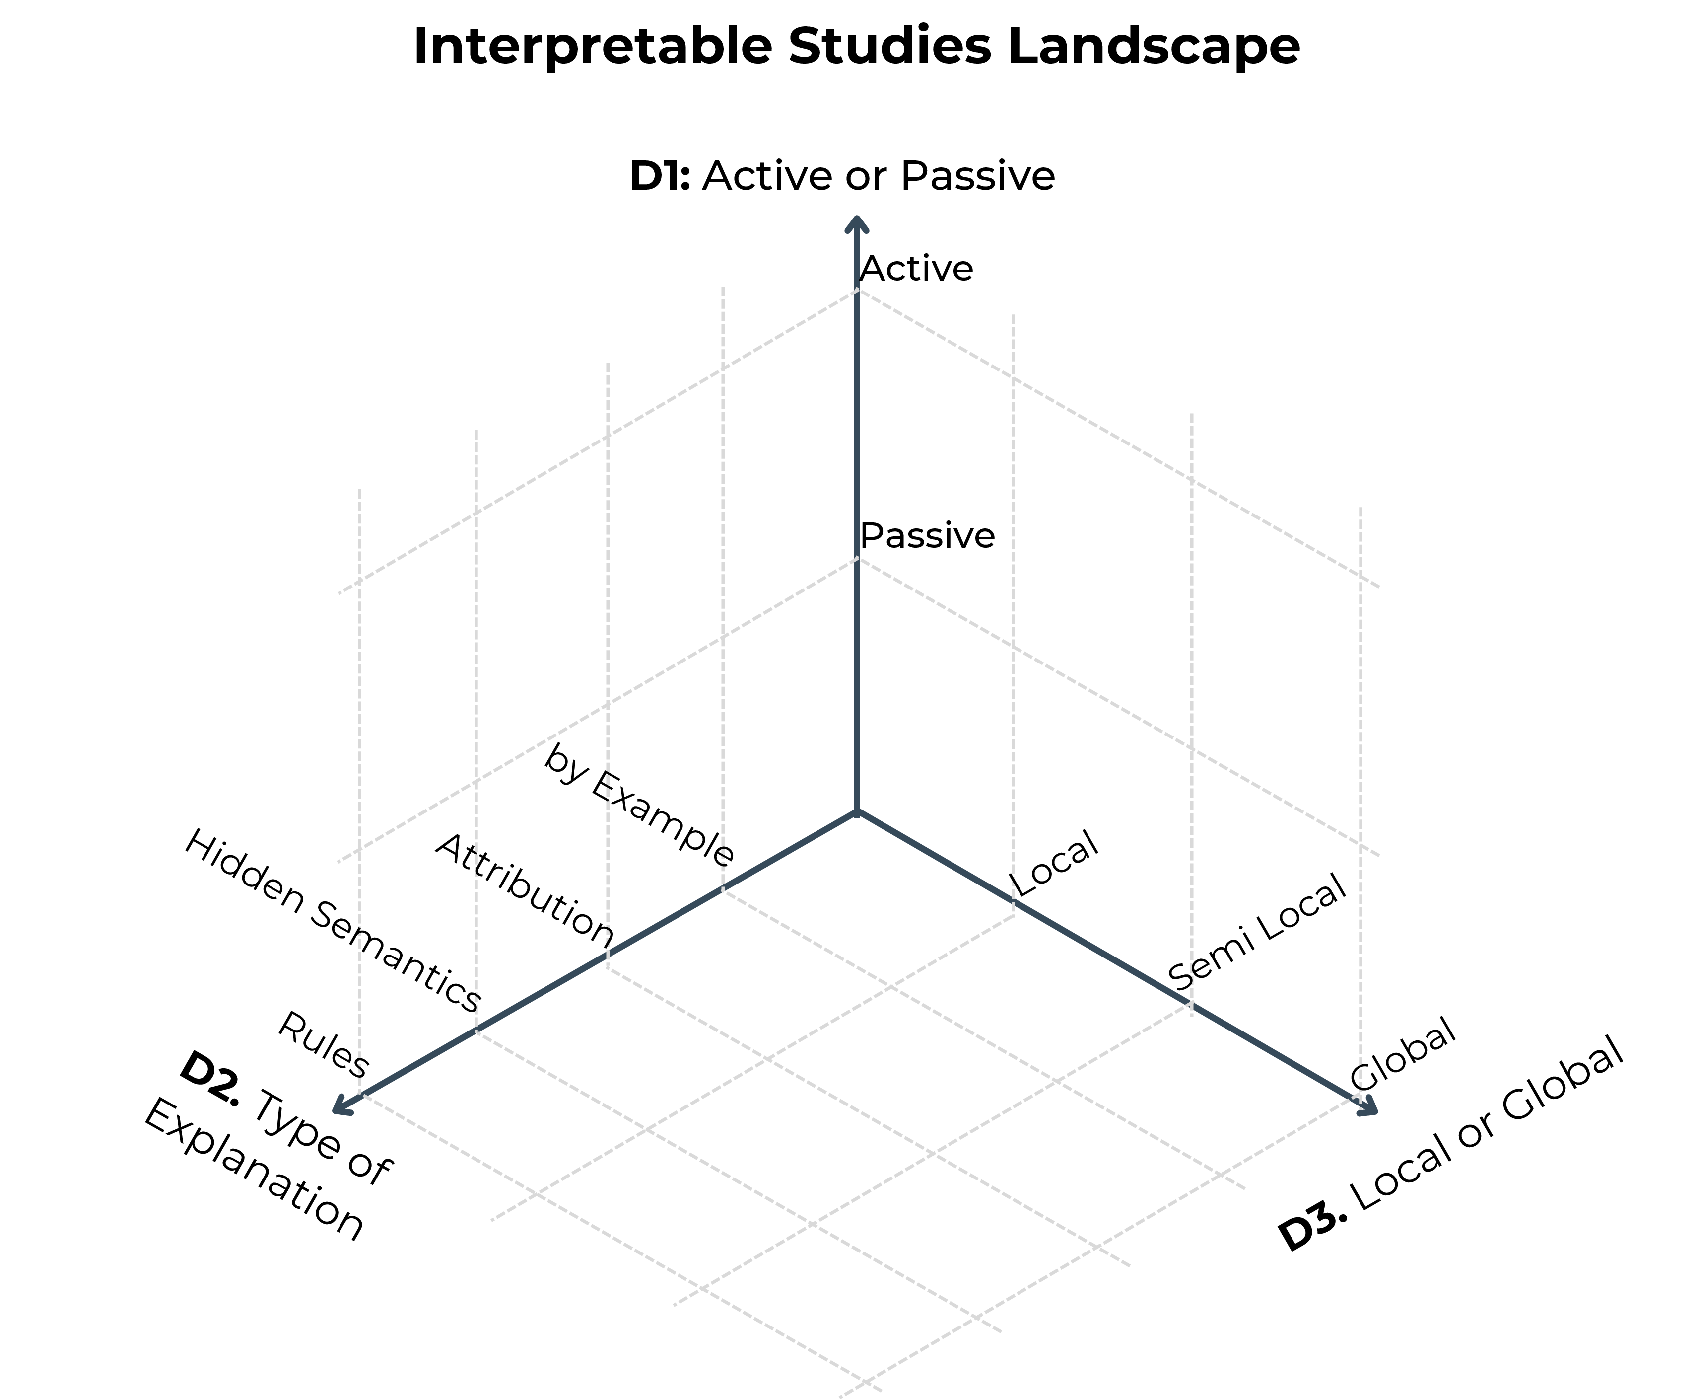
\includegraphics[width=\textwidth]{fig/rel/interp/img/dims/dreidim.pdf}
            \end{center}
    \end{columns}
    \footnotetext[1]{\tiny Lipton defines Interpretability Similarly. \\Transparency or Post-hoc Interpretations}
\end{frame}
%--------------------------------------------------------------------------------------------------
\begin{frame}[c]
    \frametitle{Interpretability}
    \framesubtitle{Post-hoc Interpretability}
    \begin{center}
        \scalebox{.75}{
    %% Definitions
    \def\posthoccirc{(0,0) circle (3.75cm)}
    \def\lrcirc{(0.8838834764831843cm, -0.8838834764831843cm) circle (2.5cm)}
    \def\attcirc{(1.7677669529663687, -1.7677669529663687) circle (1.25cm)}
    \def\gradcirc{(-0.8838834764831843, -0.8838834764831843) circle (2.5cm)}
    \def\maskcirc{(0.8838834764831843, 0.8838834764831843) circle (2.5cm)}
    \def\camcirc{(0.8838834764831843, 0.8838834764831843) circle (2.5cm)}
    %\def\xaicirc{(-2, -3) circle (3.75)}
    \begin{tikzpicture}
        \begin{scope}
            %% Anchors
            \filldraw[color=blue, fill=blue!5, opacity=0.5] \posthoccirc;
            \node[] at (0, 4) (aitxt) {Post-hoc Interpretability};\pause
            \node[] at (0.8838834764831843, 1.8661165235168156) (mltxt) {\scriptsize Learning Based Approaches};
            \filldraw[color=purple, fill=purple!5, opacity=0.5] \lrcirc; \pause
            \node[] at (0.8838834764831843, 3.6338834764831844) (nlptxt) {\scriptsize Attention Based Approaches};
            \filldraw[color=green, fill=green!5, opacity=0.5] \attcirc; \pause
            \node[] at (-0.8838834764831843, 1.8661165235168156) (cvtxt) {\scriptsize Gradient-Based Approaches};
            \filldraw[color=red, fill=red!5, opacity=0.5] \gradcirc;\pause
            \node[] at (1.7677669529663687, -0.26776695296636865) (dltxt) {\scriptsize Mask/Perturbation Based Approaches};    
            \filldraw[color=cyan, fill=cyan!5, opacity=0.5] \maskcirc;\pause
            \filldraw[color=orange, fill=orange!5, opacity=0.5] \camcirc;
            %% Text Nodes            
            %\pause
            %\filldraw[color=orange, fill=orange!5, opacity=0.5] \camcirc;
            %\node[] at (-2, -7) (xaitxt) {xAI};
            %\pause
            %% Intersection node
            %\begin{scope}
            %    \clip \dlcirc;
            %    \clip \xaicirc;
            %    \fill[color=red] \cvcirc;
            %\end{scope}
            %------------------------------------------------------------------------
            %\begin{scope}
            %    \clip \dlcirc;
            %    \clip \nlpcirc;
            %    \fill[color=orange!5, opacity=0.5] \xaicirc;;
            %\end{scope}

            %\node[] at (1, -1.25) (empt_1) {};
            %\node[] at (5, -1.25) (exp) {This study!};
            %\draw[->] (empt_1.center) -- node{} (exp.west);
        \end{scope}
\end{tikzpicture} 
}
    \end{center}
\end{frame}